\chapter{Proceso de Negocio}
El modelado del proceso de negocio permite representar de manera estructurada las actividades involucradas en el concurso de personal, identificando la interacción entre actores, flujos de trabajo y elementos del negocio.

\section{Modelado del Proceso de Negocio}
El modelado del proceso de negocio permite representar de manera estructurada y visual las actividades involucradas en el "Concurso de Personal" de Tambo. A través de la notación UML, se identifica la interacción entre actores externos, trabajadores internos, flujos de información y documentos clave.
En este apartado se presentan los modelos estructurales que definen el ecosistema del negocio:

\begin{figure}[htbp]
\centering
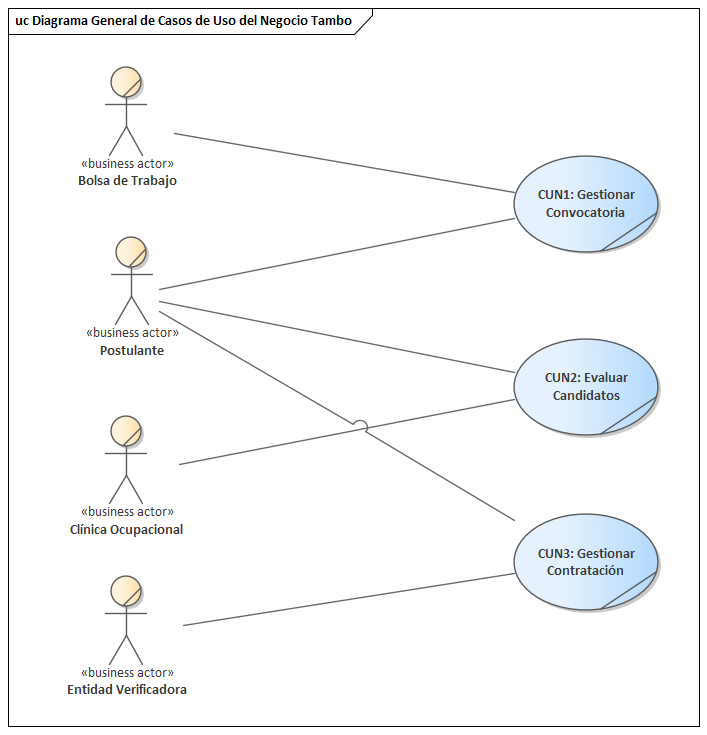
\includegraphics[width=0.7\textwidth]{figures/cun.png}
\caption{Diagrama de casos de uso del proceso de negocio}
\label{fig:casos_de_uso_de_negocio}
\end{figure}

\begin{figure}[htbp]
\centering
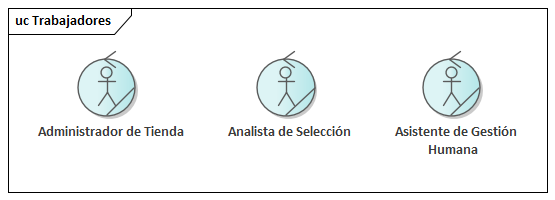
\includegraphics[width=0.7\textwidth]{figures/trabajadores.png}
\caption{Trabajadores involucrados en el proceso de negocio}
\label{fig:trabajadores_sistema_negocio}
\end{figure}

\begin{figure}[htbp]
\centering
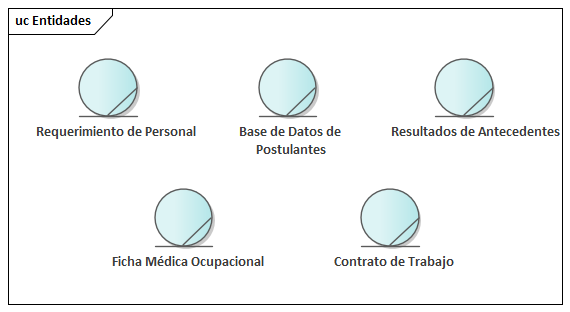
\includegraphics[width=0.7\textwidth]{figures/entidades.png}
\caption{Entidades del proceso de negocio}
\label{fig:entidades_sistema_negocio}
\end{figure}

\section{Análisis del Proceso Actual (AS-IS)}
El análisis del proceso actual (AS-IS) mapea la forma en que Tambo lleva a cabo el reclutamiento de personal sin la intervención del sistema propuesto, evidenciando cuellos de botella y vulnerabilidades operativas.

\begin{itemize}
    \item \textbf{Triaje ineficiente}: Excesivo tiempo invertido en la revisión manual y lectura de currículos físicos o correos desorganizados.
    \item \textbf{Silos de información}: Falta de una base de datos centralizada, lo que obliga a las tiendas a manejar sus propios registros en hojas de cálculo aisladas.
    \item \textbf{Trazabilidad nula}: Dificultad para que los Jefes de Tienda hagan seguimiento en tiempo real del estado de sus candidatos (si pasaron el filtro o el examen médico).
    \item \textbf{Fugas de talento}: Riesgo de perder candidatos calificados debido a la lentitud en la coordinación de entrevistas y firma de contratos.
\end{itemize}

Estas limitaciones operativas afectan la capacidad de respuesta de Tambo frente a su ritmo de expansión y apertura de nuevas tiendas.

\begin{figure}[htbp]
\centering
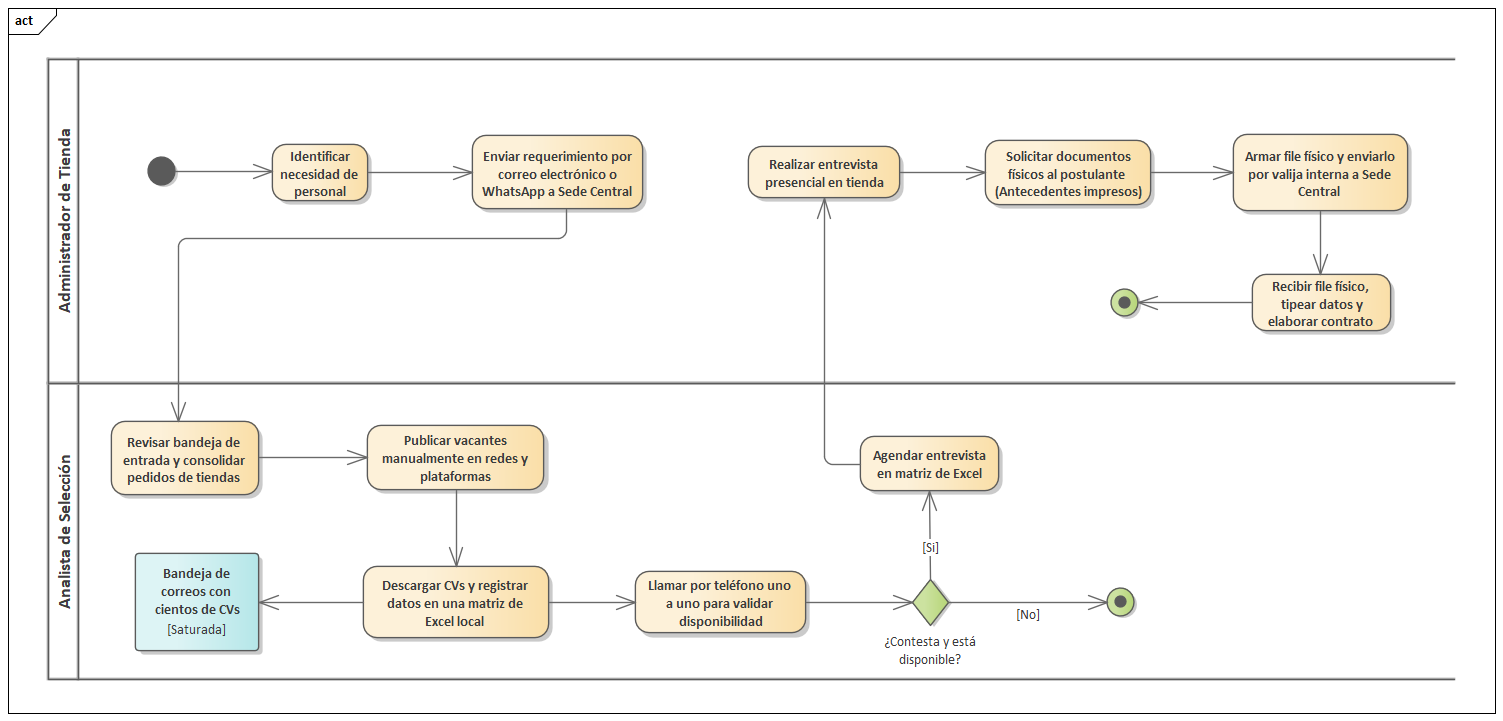
\includegraphics[width=0.7\textwidth]{figures/As-Is.png}
\caption{Diagrama AS-IS del proceso de negocio}
\label{fig:as_is_sistema_negocio}
\end{figure}

\section{Propuesta de Mejora del Proceso (TO-BE)}
La propuesta de mejora (TO-BE) plantea la reingeniería del proceso de selección mediante la implementación de un prototipo de sistema de gestión de talento. Esta solución tecnológica busca automatizar tareas repetitivas, asegurar la trazabilidad y reducir el Time-to-Hire (tiempo de contratación).

Las optimizaciones implementadas en el nuevo flujo incluyen:

\begin{itemize}
    \item \textbf{Filtro automatizado}: Pre-calificación de postulantes antes de la intervención manual del Analista de Selección.
    \item \textbf{Persistencia de datos}: Centralización de la información en un repositorio único (Base de Datos de Postulantes) accesible para Sede Central y Tiendas.
    \item \textbf{Gestión de estados}: Transición digital de los documentos (Requerimientos, CVs, Contratos) con control de versiones (Borrador, Aprobado, Firmado).
    \item \textbf{Sincronización de tareas}: Ejecución en paralelo de las verificaciones de antecedentes y exámenes médicos.
\end{itemize}

A continuación, se presentan las Realizaciones del Negocio (diagramas de actividad) que detallan el flujo de trabajo optimizado (TO-BE):

\begin{figure}[htbp]
\centering
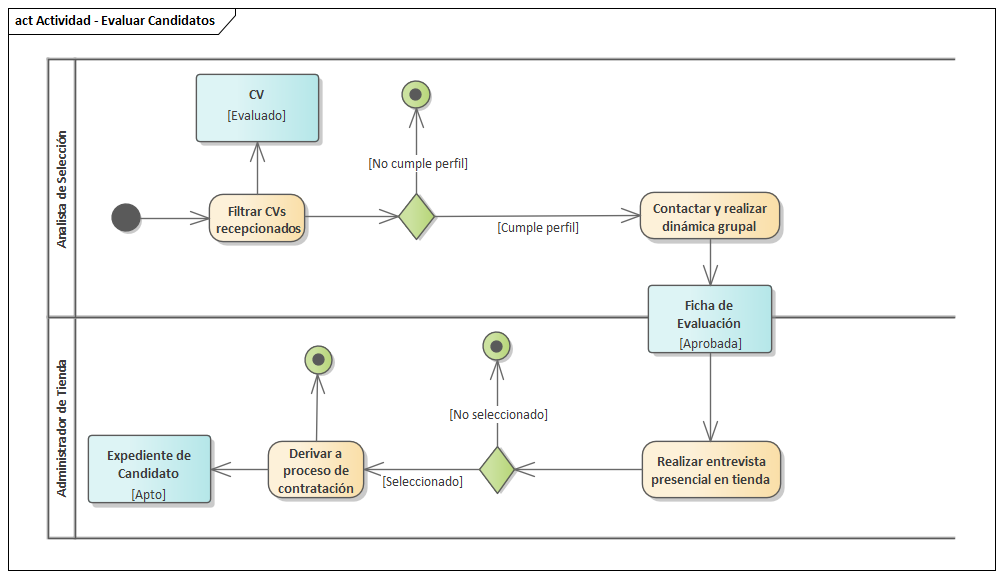
\includegraphics[width=0.7\textwidth]{figures/Actividad - Evaluar Candidatos.png}
\caption{Actividad - Evaluar Candidatos}
\label{fig:evaluar_candidatos}
\end{figure}

\begin{figure}[htbp]
\centering
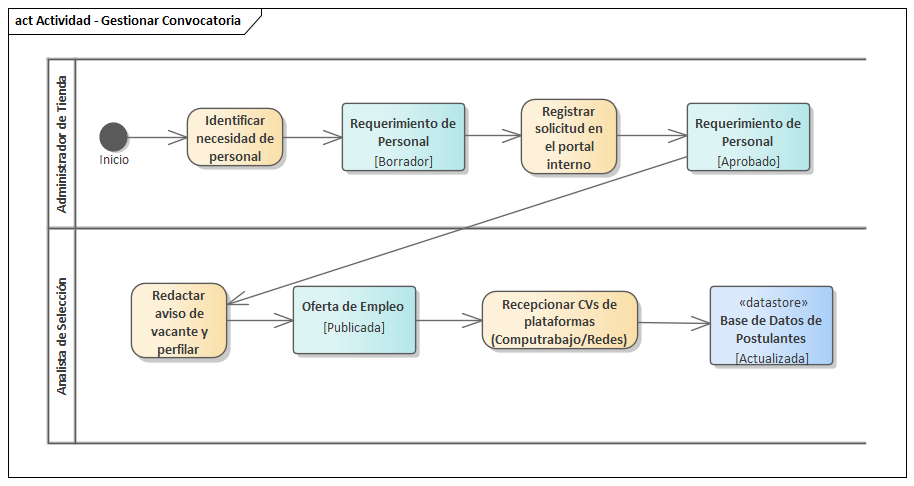
\includegraphics[width=0.7\textwidth]{figures/Actividad - Gestionar Convocatoria.png}
\caption{Actividad - Gestionar Convocatoria}
\label{fig:gestionar_convocatoria}
\end{figure}

\begin{figure}[htbp]
\centering
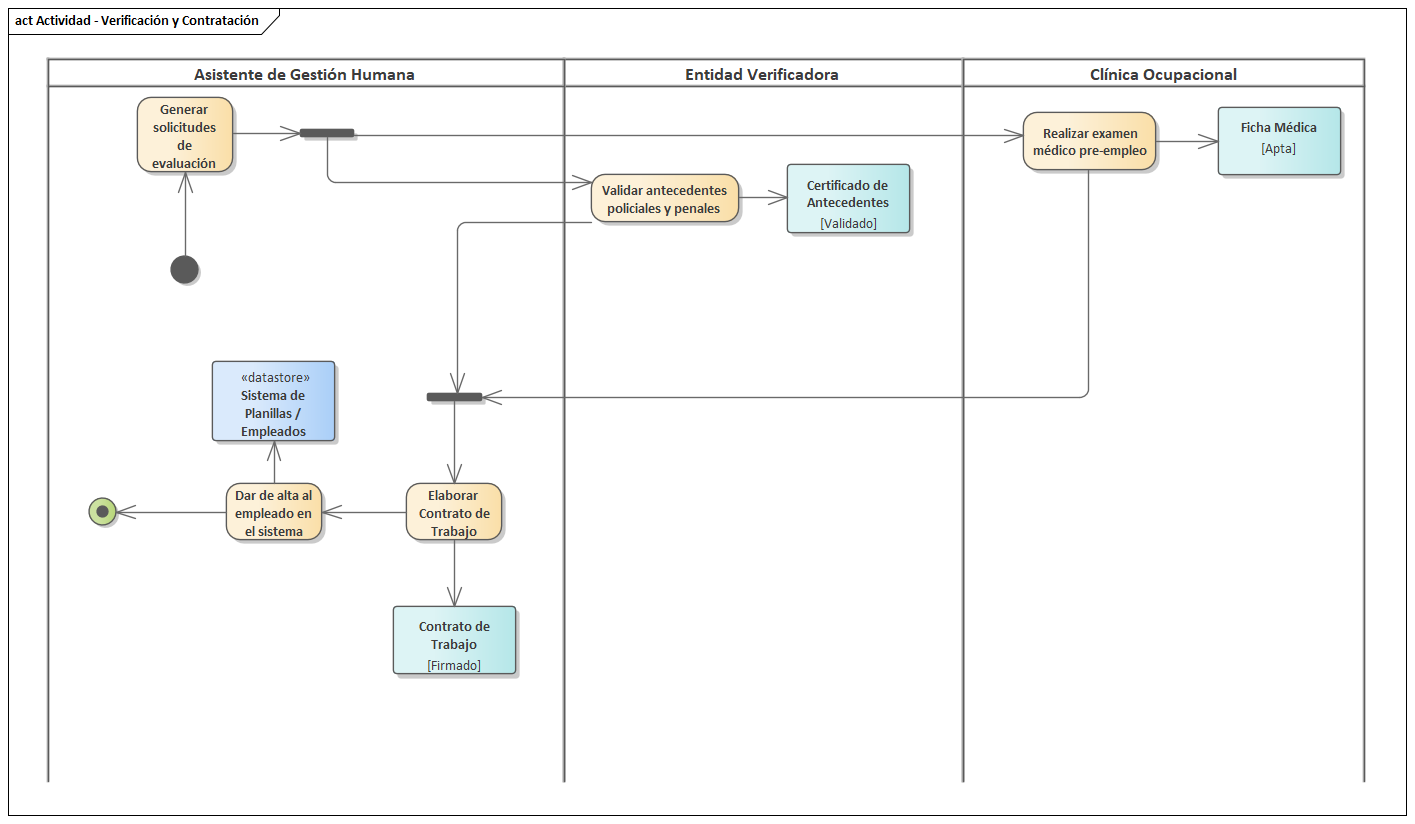
\includegraphics[width=0.7\textwidth]{figures/Actividad - Verificación y Contratación.png}
\caption{Actividad - Verificación y Contratación}
\label{fig:verificacion_contratacion}
\end{figure}

\FloatBarrier